Mosaico is a free and open-source platform that enables users and developers to create, share, and display custom content on an LED matrix. These pieces of content, called \textbf{widgets}, can be uploaded to the \textbf{widget store} for others to browse, download, and install on their personal matrix devices.

Developers can mark their widgets as \textbf{configurables}, allowing users to submit multiple configurations for the same widget. For example, an image widget can be configured to display different images based on user input.

Some examples of widgets:\footnote{Screenshots taken from the Mosaico simulator, not the actual LED matrix device}

\begin{figure}[h]
    \centering
    \begin{minipage}[b]{0.24\textwidth}
        \centering
        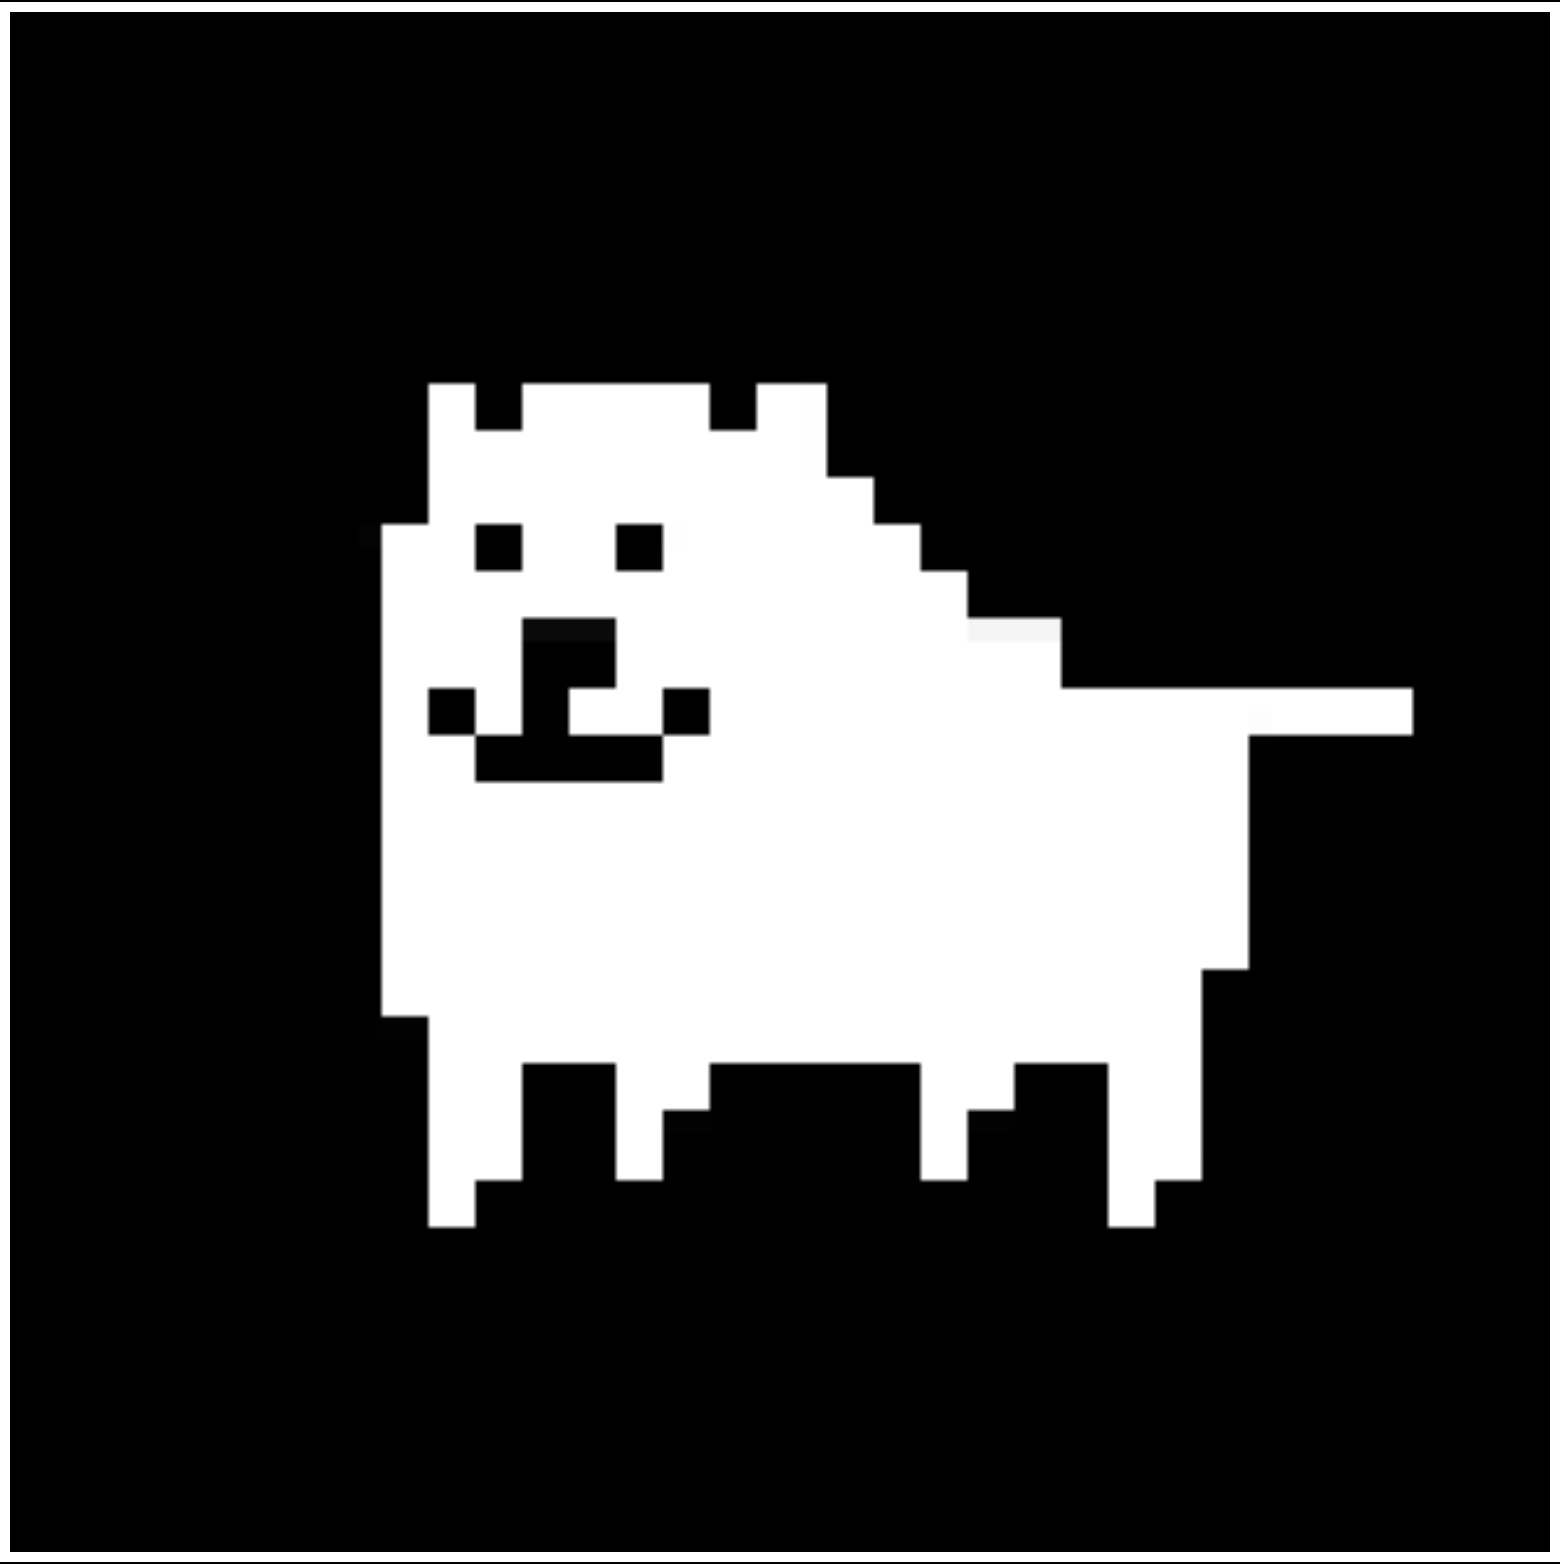
\includegraphics[width=\textwidth]{tesi/img/stylized_widgets/image.png}
        \caption*{\href{https://github.com/mosaico-widgets/image-widget}{Image} }
    \end{minipage}
    \begin{minipage}[b]{0.24\textwidth}
        \centering
        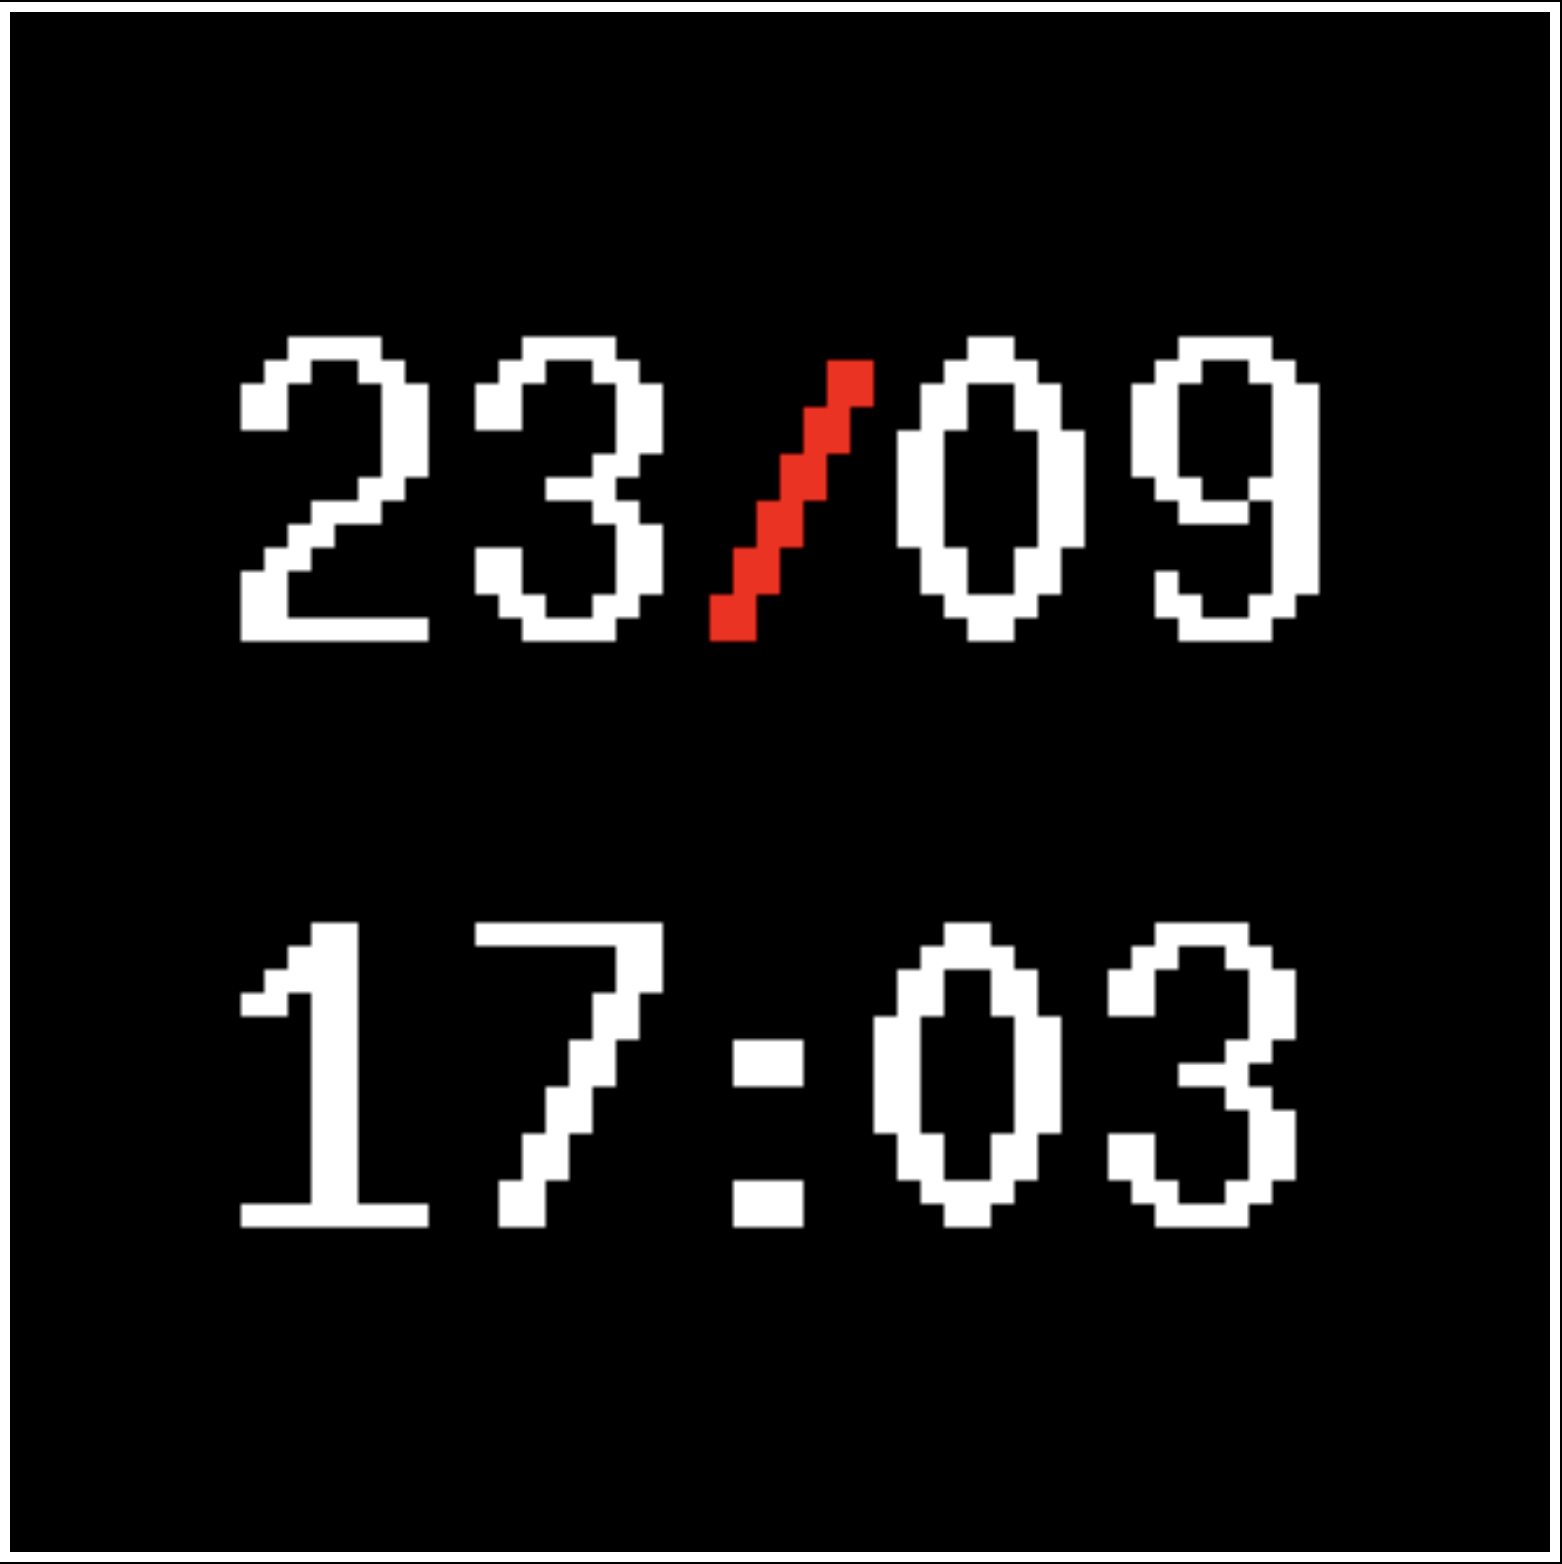
\includegraphics[width=\textwidth]{tesi/img/stylized_widgets/datetime.png}
        \caption*{\href{https://github.com/mosaico-widgets/date-and-time}{Date and Time} }
    \end{minipage}
    \begin{minipage}[b]{0.24\textwidth}
        \centering
        
\includegraphics[width=\textwidth]{tesi/img/stylized_widgets/dice.png}
        \caption*{\href{https://github.com/mosaico-widgets/d6}{Dice roll} }
    \end{minipage}
    \begin{minipage}[b]{0.24\textwidth}
        \centering
        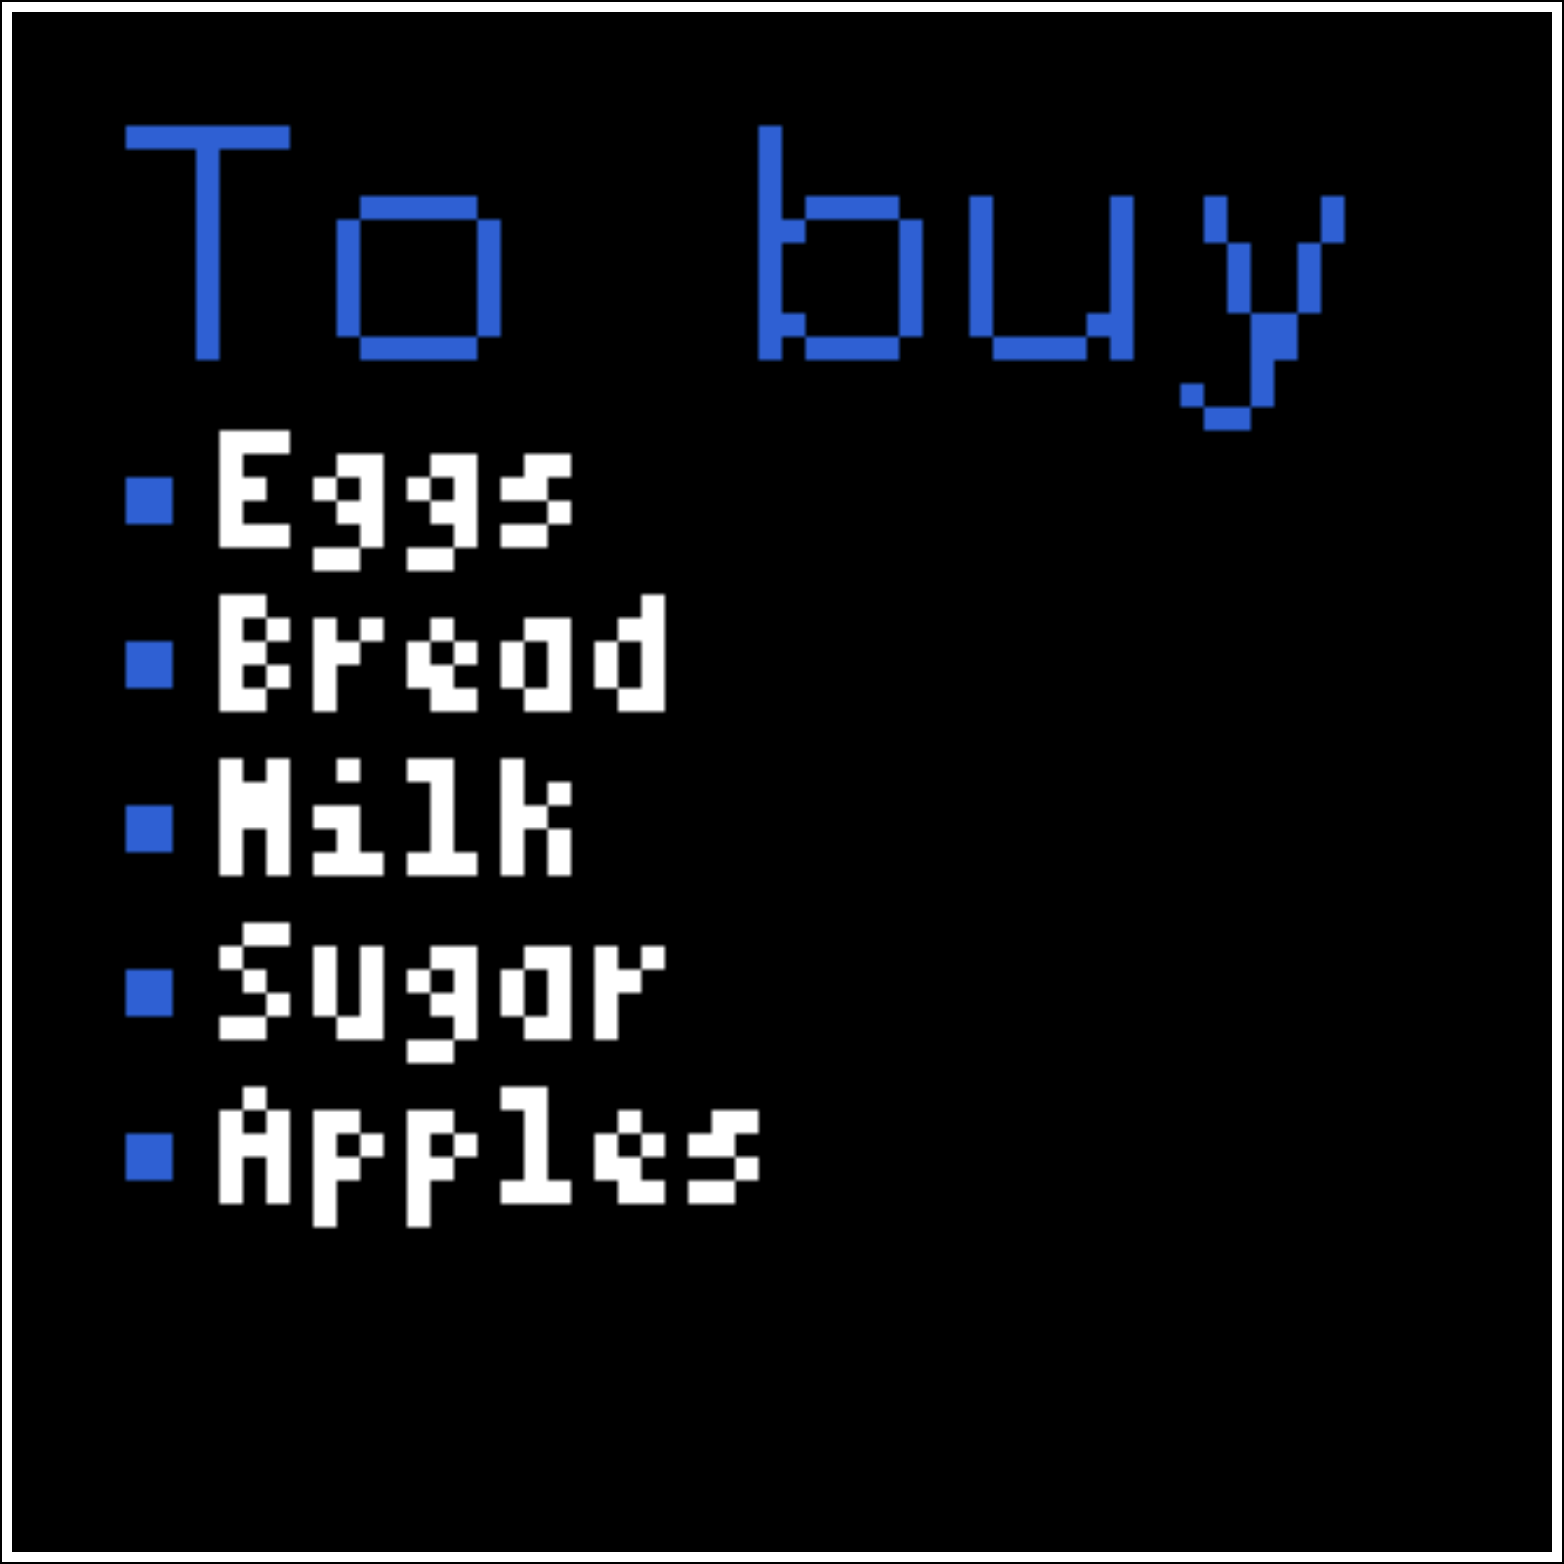
\includegraphics[width=\textwidth]{tesi/img/stylized_widgets/lists.png}
        \caption*{\href{https://github.com/mosaico-widgets/list}{List} }
    \end{minipage}
\end{figure}

The platform consists of multiple applications that work together seamlessly to deliver dynamic, customizable content to a Raspberry Pi-driven LED matrix.

\section{Motivation}
The growing demand for interconnected devices capable of communication in constrained environments has fueled the rapid expansion of the Internet of Things (IoT). As a tech enthusiast, I was naturally drawn to this world when I moved into my own home, where I sought to make every electronic device “smart” futhermore, I have always enjoyed having control centralized in a single place, like a dashboard—somewhere I can display dynamic information for everything I want to monitor.

Nevertheless, building a real-time content display system in an IoT environment presents several challenges, such as constrained bandwidth and low computational power. This thesis focuses on overcoming these obstacles by developing an IoT-based display system that leverages CoAP and BLE to efficiently deliver real-time dynamic content to an LED matrix driven by a Raspberry Pi.



\section{Open Source}
The Mosaico project has been developed and released under the AGPL-3.0 license, a copyleft open-source license designed to ensure that modifications and derivative works are freely available to the community. The full project code, including the various components of the platform, is publicly accessible for review, modification, and redistribution. The project's source code is organized and hosted on GitHub and can be found at the following \footnote{\url{https://github.com/orgs/mosaico-matrix}}. Additionally, a separate organization dedicated to the collection and publication of community-created widgets is available \footnote{\url{https://github.com/orgs/mosaico-widgets/}}.

Open-source software plays a pivotal role in advancing technological innovation and promoting collaborative development. By adopting an open-source model, Mosaico not only enables users to benefit from the transparency and adaptability of the software but also fosters an ecosystem where developers and hobbyists alike can contribute enhancements, fix bugs, and create new functionalities that serve the needs of the broader community. This collective effort accelerates the development process, often yielding more secure, stable, and feature-rich software than proprietary alternatives.

Furthermore, the Mosaico ecosystem is designed to embrace these open-source values not only in the core platform but also in the development and sharing of widgets. 

By leveraging the open-source model, Mosaico aspires to build a self-sustaining, innovative community that thrives on shared knowledge and collective growth.